\chapter{Théorie des graphes et algorithmes}
\section{Parcours d'un graphe}
\subsection{Le parcours en profondeur}
La DFS ou Depth-First Search  est la méthode la plus simple pour parcourir un graphe. Elle fonctionne sur tout type de graphe, cyclique ou non,orienté ou non.

Le procédure de parcours pour la DFS n'est pas le même pour un graphe orienté et pour un graphe non orienté.

\subsubsection{DFS pour graphe non orienté}
En principe, on choisit un sommet r racine pour démarrer la recherche ou le parcours. Puis on traverse l'arête e = (r,v) qui menè vers le sommet v. En même temps on oriente e de r vers v. Maintenant, on dit que l'arête e examiné et on l'appelle arête d'un arbre.
Le sommet r est appelé père de v et on dénote r=pere(v). On continue la recherche ou le parcours.
Au sommet x, il y a deux cas:
\begin{enumerate}
	\item si tout les arêtes incident à x ont été examiné, on retourne vers le pere de x et on continue le processus sur pere(x). On dit que le sommet x est complètement examiné.
	\item s'il existe un ou plusieurs arête(s) non examiné incident à x, alors on choisit un de ces arête e = (x,y) et on l'oriente de x vers y. Maintenant cet arête est dit "a examiné". On a deux sous cas maintenant:
	\begin{enumerate}
		\item Si y n'a pas encore été visité, on travers l'arête (x,y), on visite y et le parcours continue sur y. Dans ce cas, e = (x,y) est un arête de l'arbre et pere(y) = x.
		\item Si y a été visité auparavant, on sélectionne d'autres arêtes non examiné de x. Dans ce cas, e = (x,y) est appelé arête de retour.  
	\end{enumerate} 
\end{enumerate}
A chaque fois qu'on arrive à un nouveau sommet qui n'était pas encore visité, on lui donne un numero unique. Le numero de la racine est 1.
$$DFN(x)=numero\ courant\ du\ sommet\ x$$ 

Une DFS complète stop quand on revient à la racine et on a déjà visité tout les sommets ou quand on a trouvé le sommet/arête désiré.

La DFS divise les arêtes du graphe G en arêtes d'arbre et arêtes de retour. Manifestement, les arêtes d'arbre forme un arbre étendu de G aussi connu sous le nom de arbre de la DFS. Si on inclut les orientations des arêtes de l'arbre, on obtient un arbre orienté de la DFS. 
\begin{figure}
\centering
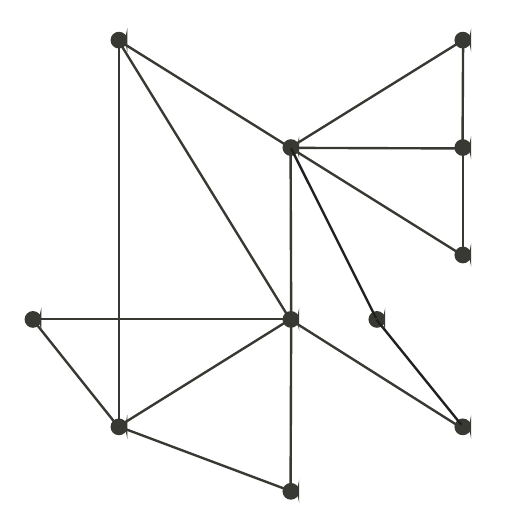
\includegraphics[width=0.3\linewidth]{images/dfs-search-example}
\caption{Graphe non-orienté: parcours DFS}
\label{fig:dfs-search-example}
\end{figure}

Pour la figure \ref{fig:dfs-search-example}, on débute la DFS sur le sommet au coin supérieur gauche.
L'arbre de la DFS correspondant est représenté par la figure 
\begin{figure}
\centering
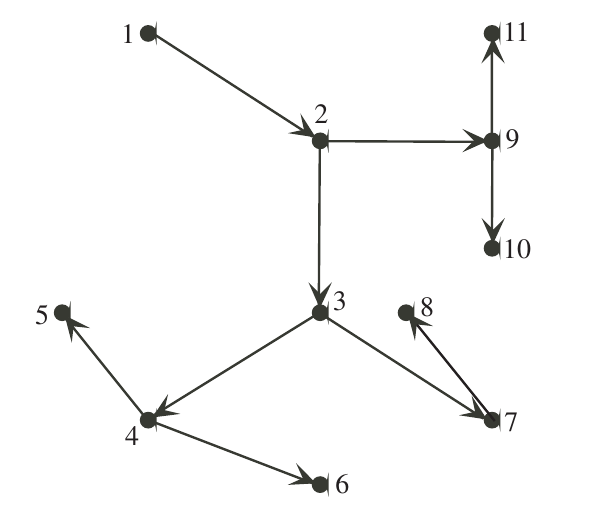
\includegraphics[width=0.3\linewidth]{images/dfs-tree-non-directed}
\caption{Arbre de la DFS correspondant au graphe non orienté \ref{fig:dfs-search-example}}
\label{fig:dfs-tree-non-directed}
\end{figure}


Dans la suite, on dénote par
\begin{equation*}
 K(x)=\left\{
 \begin{array}{l l}
 0 & \quad \text{si le sommet x n'a pas été visité}\\
 1 & \quad \text{si le sommet x a été visité}
 \end{array} \right.
\end{equation*}

et ARBRE et RETOUR sont des variables contenant les 
arêtes orientés de l'arbre et les arêtes de retour.


On peut donc représenté l'algorithme comme suit:

\begin{algorithm}
\caption{Depth First Search: graphe non orienté}
\begin{algorithmic}
\State $ARBRE \gets \emptyset$
\State $RETOUR \gets \emptyset$



\end{algorithmic}
\end{algorithm}

\begin{verbatim}
ARBRE = []
RETOUR = []
i = 1
pour tout sommet de G
	sommet.pere = 0
	sommet.k = 0
fin pour

\end{verbatim}
\begin{enumerate}
	\item Mettre  $ARBRE \longleftarrow\ \emptyset\ et\ i\longleftarrow\ 1$, 
\end{enumerate}


 
 